\section{Compactness for Sets of Regular Patterns}

In this section, we define the compactness of sets of regular patterns, formally.
Then, if $\sharp\Sigma \ge 2k-1$ holds, 
we show that 
$\RPat^{k}$ has compactness with respect to the containment.

\begin{dfn}
Let $\mathcal{C}$ be a subset of $\RPatplus$ (resp. $\Patplus$). 
For any regular pattern $p \in \RPat$ (resp. $\Pat$) and any set $Q \in \mathcal{C}$,
the set $\mathcal{C}$ has compactness with respect to containment.
\end{dfn}

\begin{lem}[Sato et al.\cite{Sato1}]\label{変数2つ}
Let $\Sigma$ be an alphabet with $\Sigma \ge 3$ and $p,q$ regular patterns on $\Sigma$.
Let $D$ be the set of either $(\mathrm{i})$ or $(\mathrm{ii})$ of regular patterns on $\Sigma$ below: Assume that $a \not= b$ and that a variable symbol $y$ does not appear in $p$.
\begin{align*}
(\mathrm{i})~~\{ ay, by \}~~~(\mathrm{ii})~\{ ya, yb \}.
\end{align*}
Then, if $p \{ x := r \} \preceq q$ for all $r \in D$, then $p \{ x := xy \} \preceq q$.
\end{lem}
\begin{proof}
It is obvious if no variable symbol appears in $p$. 
Therefore, let $p=p_{1}xp_{2}$, where $p_{1}, p_{2}$ are regular patterns and $x$ is a variable symbol.
We assume that $p \{ x := xy \} \not \preceq q$ in order to derive the contradictions.

\noindent
(i) 
The case of $D=\{ ay, by \} \ (a \ne b)$.

\noindent
Since $p \{ x := xy \} \not \preceq q$, $p_{1}ayp_{2}\preceq q$ and $p_{1}byp_{2}\preceq q$, 
there exist regular patterns $q_{1},q_{2}$ on $\Sigma$ such that $q=q_{1}ay_{1}wby_{2}q_{2}$ or $q=q_{1}by_{1}way_{2}q_{2}$ for some variable symbols $y_{1},y_{2}~(y_{1} \not= y_{2})$ and a constant string $w$ ($|w|\geq 0$) from Theorem \ref{Sato1:Lemma9}.
When $q=q_{1}ay_{1}wby_{2}q_{2}$ holds, the following four equations (1), (2), (1'), (2') holds:
\begin{align*}
\textrm{(1)} & ~p_{1} \preceq q_{1}\\
\textrm{(1')} & ~p_{2} \preceq wby_{2}q_{2} \mbox{ or } p_{2} \preceq y^{\prime}wby_{2}q_{2} ~~(y^{\prime} \in X)\\
\textrm{(2)} & ~p_{1} \preceq q_{1}ay_{1}w\\
\textrm{(2')} & ~p_{2} \preceq q_{2} \mbox{ or } p_{2} \preceq y^{\prime\prime}q_{2} ~(y^{\prime\prime} \in X)
\end{align*}
From the above equation (2), there exist regular patterns $p_{1}^{\prime},p_{1}^{\prime\prime}$ such that $p_{1}=p_{1}^{\prime}p_{1}^{\prime\prime}$, $p_{1}^{\prime} \preceq q_{1}a$ and $p_{1}^{\prime\prime} \preceq y_{1}w$ hold.
Therefore, since $p=p_{1}xp_{2}=p_{1}^{\prime}p_{1}^{\prime\prime}xp_{2}$,
if $p_{2} \preceq wby_{2}q_{2}$ holds, 
$p\preceq q_{1}ap_{1}^{\prime\prime}xwby_{2}q_{2}=q \{ y_{1} := p_{1}^{\prime\prime}x \}$ holds.
Otherwise, that is $p_2\preceq y'wby_{2}q_{2}$, $p\preceq q_{1}ap_{1}^{\prime\prime}xy'wby_{2}q_{2}=q \{ y_{1} := p_{1}^{\prime\prime}xy' \}$ holds.
Hence, $p \preceq q$ holds.
This contradicts the assumption.

\noindent
(ii) 
The case of $D=\{ ya, yb \} \ (a \ne b)$.
By reversing the strings of $p$ and $q$, we can prove that $p \{ x := xy \} \preceq q$ holds, in a similar way as (i).
\end{proof}

\begin{lem}\label{補題14}
Let $\Sigma$ be an alphabet with $\Sigma \ge 4$, $p,q$ regular patterns on $\Sigma$.
Let $D$ be the following set of constant strings on $\Sigma$ whose lengths are just 2:

\medskip
\noindent
~~\begin{tabular}{l}
  $D = \{ a_{1}b_{1}, a_{2}b_{2}, a_{3}b_{3}, a_{4}b_{4} \}$\\
  $(a_{i} \ne a_{j} \mbox{ and } b_{i} \ne b_{j} \mbox{ for each } i,j~(i\ne j, 1\ge i,j\ge 4))$.
\end{tabular}
\medskip

\noindent
We assume that a variable symbol $y$ does not appear in $p$.
Then, if $p \{ x := r \} \preceq q$ for all $r \in D$, then $p \{ x := xy \} \preceq q$.  
\end{lem}
\begin{proof}
It is obvious if the variable symbol $x$ does not appear in $p$.
Therefore, let $p=p_{1}xp_{2}$, where $p_{1}, p_{2}$ are regular patterns.
We assume that $p \{ x := xy \} \not \preceq q$ in order to derive the contradictions.
Since $p \{ x := r \} \preceq q$ holds for any $r \in D$,
the regular pattern $q$ contains $a_{1}b_{1}, a_{2}b_{2}, a_{3}b_{3}$, and $a_{4}b_{4}$.
We remark that $a_i$ and $b_j$ may be same for $i,j (1\le i,j\le 4)$.
Since $p \{ x := r \} \preceq q$ for all $r \in D$ holds, 
there exist the following 15 cases (i)--(xv) for four regular patterns on $\Sigma$ contained in $q$ that correspond to four constant strings in $D$:
Here, $y_1,y_2,y_3,y_4$ are variable symbols.

\medskip  

\noindent
\begin{tabular}{ll}
(i)~~~~$a_{1}b_{1}, a_{2}b_{2}, a_{3}b_{3}, a_{4}b_{4}$  & (ix)~~~ $a_{1}b_{1}, y_{1}b_{2}, a_{3}y_{2}, a_{4}y_{3}$ \\
(ii)~~~$a_{1}b_{1}, a_{2}b_{2}, a_{3}b_{3}, a_{4}y_{1}$  & (x)~~~~ $a_{1}b_{1}, a_{2}y_{1}, a_{3}y_{2}, a_{4}y_{3}$ \\
(iii)~~$a_{1}b_{1}, a_{2}b_{2}, a_{3}b_{3}, y_{1}b_{4}$ & (xi)~~~ $y_{1}b_{1}, y_{2}b_{2}, y_{3}b_{3}, y_{4}b_{4}$ \\
(iv)~~~$a_{1}b_{1}, a_{2}b_{2}, a_{3}y_{1}, y_{2}b_{4}$  & (xii)~~ $y_{1}b_{1}, y_{2}b_{2}, y_{3}b_{3}, a_{4}y_{4}$ \\
(v)~~~~$a_{1}b_{1}, a_{2}b_{2}, y_{1}b_{3}, y_{2}b_{4}$    & (xiii)~ $y_{1}b_{1}, y_{2}b_{2}, a_{3}y_{3}, a_{4}y_{4}$ \\
(vi)~~~$a_{1}b_{1}, a_{2}b_{2}, a_{3}y_{1}, a_{4}y_{2}$   & (xiv)~~$y_{1}b_{1}, a_{2}y_{2}, a_{3}y_{3}, a_{4}y_{4}$ \\
(vii)~~$a_{1}b_{1}, y_{1}b_{2}, y_{2}b_{3}, y_{3}b_{4}$  & (xv)~~~$a_{1}y_{1}, a_{2}y_{2}, a_{3}y_{3}, a_{4}y_{4}$ \\
(viii)~$a_{1}b_{1}, y_{1}b_{2}, y_{2}b_{3}, a_{4}y_{3}$ &        %& ($y_{1},y_{2},y_{3},y_{4}$は変数記号)
\end{tabular}
\medskip

\noindent
For the cases (v)--(xv), we can prove that $p \{ x := xy \} \preceq q$ holds in a similar way as Lemma \ref{変数2つ}.
Hence, for the cases (i)--(iv), we will prove that $p \{ x := xy \} \preceq q$ holds.

\smallskip
\noindent
(I) Cases of (i), (ii) and (iii), that is the cases that $q$ contains $a_{1}b_{1}, a_{2}b_{2}$ and $a_{3}b_{3}$:

\begin{figure}
\centering
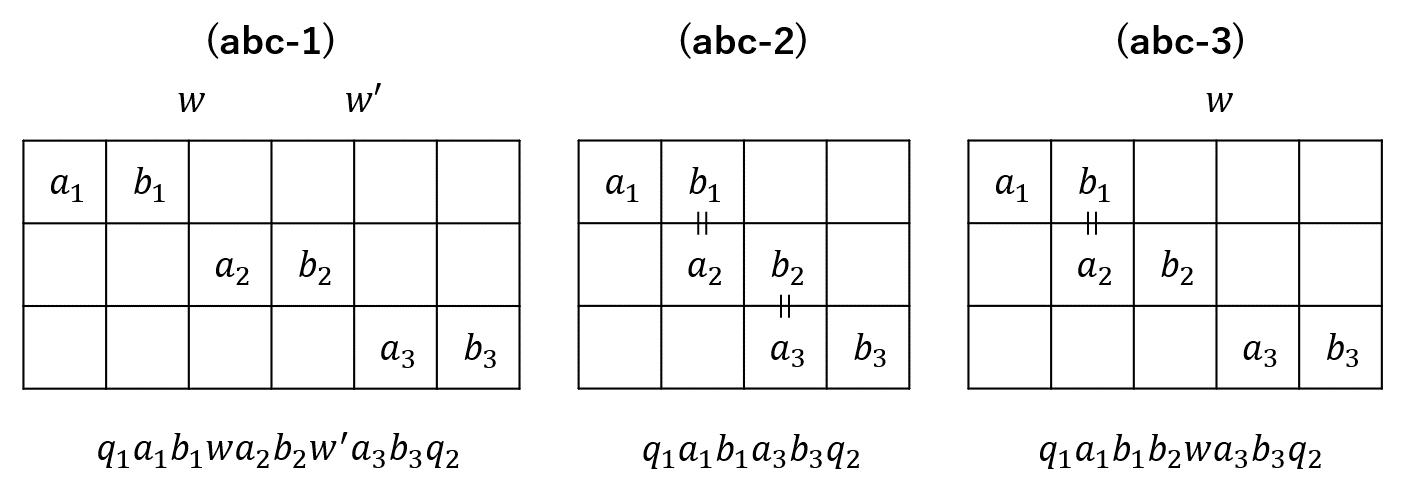
\includegraphics[width=\linewidth]{figs/Cases-abc.png}
\vspace{-1cm}
\caption{(abc)の場合分け}
\label{abc組み合わせ}
\end{figure}

\noindent
We consider the following three cases (I-1)-(I-3) of $q$ for some regular patterns $q_{1},q_{2}$ and some constant strings $w,w^{\prime}$ ($|w|\geq 0$ and $|w^{\prime}|\geq 0$):

\smallskip
\noindent
\begin{tabular}{ll}
(I-1) $q=q_{1}a_{1}b_{1}wa_{2}b_{2}w^{\prime}a_{3}b_{3}q_{2}$,\\
(I-2) $q=q_{1}a_{1}b_{1}a_{3}b_{3}q_{2}$ ($b_{1}=a_{2}$ and $a_{3}=b_{2}$),\\
(I-3) $q=q_{1}a_{1}b_{1}b_{2}wa_{3}b_{3}q_{2}$ ($b_{1}=a_{2}$)\\
(I-4) $q=q_{1}a_{1}b_{1}wa_{2}b_{2}b_{3}q_{2}$ ($b_{2}=a_{3}$).
\end{tabular}
\smallskip

\noindent
(I-1) Case of $q=q_{1}a_{1}b_{1}wa_{2}b_{2}w^{\prime}a_{3}b_{3}q_{2}$:
Assume that the following six equations (1),(2),(3),(1'),(2'),(3') are hold.
\begin{align*}
\textrm{(1)}~& p_{1} \preceq q_{1} & \textrm{(1')}~& p_{2} \preceq wa_{2}b_{2}w^{\prime}a_{3}b_{3}q_{2} \\
\textrm{(2)}~& p_{1} \preceq q_{1}a_{1}b_{1}w & \textrm{(2')}~& p_{2} \preceq w^{\prime}a_{3}b_{3}q_{2} \\
\textrm{(3)}~& p_{1} \preceq q_{1}a_{1}b_{1}wa_{2}b_{2}w^{\prime} & \textrm{(3')}~& p_{2} \preceq q_{2}
\end{align*}

If $|w|=|w^{\prime}|$ holds, $a_{1}b_{1}wa_{2}b_{2}w^{\prime}$ and $a_{1}b_{1}w$ are the suffix of $p_{1}$ from the above equations (2) and (3).
Then, $a_{1}b_{1}w=a_{2}b_{2}w^{\prime}$.
Hence, $a_{1}b_{1}=a_{2}b_{2}$.
This contracts the assumption of $a_{1} \ne a_{2}$ and $b_{1} \ne b_{2}$.

If $|w|+1=|w^{\prime}|$ holds, $wa_{2}b_{2}w^{\prime}a_{3}b_{3}$ and $w^{\prime}a_{3}b_{3}$ are the prefix of $p_{2}$.
If there exists a constant symbol $w_{1}$ such that $w^{\prime}a_{3}b_{3}=ww_{1}a_{3}b_{3}$,
then $b_{2}$ and $a_{3}$ are the same symbol from $wa_{2}b_{2}=ww_{1}a_{3}$.
From the above equations (2) and (3), $a_{1}b_{1}wa_{2}b_{2}w^{\prime}$ and $a_{1}b_{1}w$ are the suffix of $p_{1}$.
Then, there exists a constant symbol $w_{2}$ such that $w^{\prime}=w_{2}w$,
then $b_{2}$ and $a_{1}$ are the same symbol from $b_{2}w_{2}w=a_{1}b_{1}w$.
Hence, from $b_{2}=a_{3}$, $a_{3}$ and $a_{1}$ are same symbol.
This contradicts the assumption of $a_{3} \ne a_{1}$.

If $|w|+1 < |w^{\prime}|$, from the above (2) and (3), 
$a_{1}b_{1}wa_{2}b_{2}w^{\prime}$ and $a_{1}b_{1}w$ are the suffix of $p_{1}$.
If there exists a constant string $w_{1}$ ($|w_{1}|\geq 2$) such that $w^{\prime}=w_{1}w$, then $a_{2}b_{2}$ is the suffix of $w_{1}$.
From  the above equations ($1'$) and ($2'$), 
$wa_{2}b_{2}w^{\prime}a_{3}b_{3}$ and $w^{\prime}a_{3}b_{3}$ are the prefix of $p_{2}$.
If there exist constant strings $w_{1}$ and $w_{2}$ such that $w^{\prime} = w_{1}w=ww_{2}$ holds, then $a_{2}b_{2}$ and $a_{3}b_{3}$ are the suffix of $w_{1}$ from $|ww_{2}a_{3}b_{3}|=|wa_{2}b_{2}w_{1}|$.
Hence, $a_{2}b_{2}=a_{3}b_{3}$.
This contradicts the assumption of $a_{2} \ne a_{3}$ and $b_{2} \ne b_{3}$.
\smallskip

\noindent
(I-2) Case of $q=q_{1}a_{1}b_{1}a_{3}b_{3}q_{2}$ ($b_{1}=a_{2}$ and $a_{3}=b_{2}$):
Assume that the following six equations (1),(2),(3),(1'),(2'),(3') are hold.
\begin{align*}
\textrm{(1)}~& p_{1} \preceq q_{1} & \textrm{(1')}~& p_{2} \preceq a_{3}b_{3}q_{2} \\
\textrm{(2)}~& p_{1} \preceq q_{1}a_{1} & \textrm{(2')}~& p_{2} \preceq b_{3}q_{2} \\
\textrm{(3)}~& p_{1} \preceq q_{1}a_{1}b_{1} & \textrm{(3')}~& p_{2} \preceq q_{2}
\end{align*}

\noindent
From the above equations (2) and (3), since $a_{1}b_{1}$ and $a_{1}$ are the suffix of $p_{1}$, 
$b_{1} = a_{1}$ holds.
From the assumption of $b_{1}=a_{2}$, $a_{1}=a_{2}$.
This contradicts the assumption of $a_{1}\not= a_{2}$.
\smallskip

\noindent
(I-3) Case of $q=q_{1}a_{1}b_{1}b_{2}wa_{3}b_{3}q_{2}$ ($b_{1}=a_{2}$):
Assume that the following six equations (1),(2),(3),(1'),(2'),(3') are hold.
\begin{align*}
\textrm{(1)}~& p_{1} \preceq q_{1} & \textrm{(1')}~& p_{2} \preceq b_{2}wa_{3}b_{3}q_{2} \\
\textrm{(2)}~& p_{1} \preceq q_{1}a_{1} & \textrm{(2')}~& p_{2} \preceq wa_{3}b_{3}q_{2} \\
\textrm{(3)}~& p_{1} \preceq q_{1}a_{1}b_{1}b_{2}w & \textrm{(3')}~& p_{2} \preceq q_{2}
\end{align*}
%\noindent
If $|w|=0$, that is $w$ is the empty string, then $a_{1}$ and $a_{1}b_{1}b_{2}$ are the suffix of $p_{1}$ from the above equations (2) and (3)
and $b_{2}a_{3}b_{3}$ and $a_{3}b_{3}$ are the prefix of $p_{2}$ from the above equations (1') and (2').
Since $b_{2}=a_{1}$ and $b_{2}a_{3}=a_{3}b_{3}$, $a_{1}=a_{3}$ holds.
This contradicts the assumption of $a_{1}\not= a_{3}$.

%\noindent
If $|w| \ge 1$, $a_{1}$ and $a_{1}b_{1}b_{2}w$ are the suffix of $p_{1}$ from the above equations (2) and (3).
Hence, the last symbol of $w$ is $a_{1}$.
Moreover, $b_{2}wa_{3}b_{3}$ and $wa_{3}b_{3}$ are the prefix of $p_{2}$ from the above equations (1') and (2').
Hence, the last symbol of $w$ is $a_{3}$.
Therefore, $a_{1}=a_{3}$ holds.
This contradicts the assumption of $a_{1} \ne a_{3}$.
\smallskip

\noindent
(I-4) Case of $q=q_{1}a_{1}b_{1}wa_{2}b_{2}b_{3}q_{2}$ ($b_{2}=a_{3}$):
Assume that the following six equations (1),(2),(3),(1'),(2'),(3') are hold.
\begin{align*}
\textrm{(1)}~& p_{1} \preceq q_{1} & \textrm{(1')}~& p_{2} \preceq wa_{2}b_{2}b_{3}q_{2} \\
\textrm{(2)}~& p_{1} \preceq q_{1}a_{1}b_{1}w & \textrm{(2')}~& p_{2} \preceq b_{3}q_{2} \\
\textrm{(3)}~& p_{1} \preceq q_{1}a_{1}b_{1}wa_{2} & \textrm{(3')}~& p_{2} \preceq q_{2}
\end{align*}
\noindent

%\noindent
If $|w|=0$, that is $w$ is the empty string, then $a_{1}b_{1}$ and $a_{1}b_{1}a_{2}$ are the suffix of $p_{1}$ from the above equations (2) and (3)
and $a_{2}b_{2}b_{3}$ and $b_{3}$ are the prefix of $p_{2}$ from the above equations (1') and (2').
Since $b_{1}=a_{2}$ and $a_{2}=b_{3}$, then $b_{1}=b_{3}$ holds.
This contradicts the assumption of $b_{1}\not= b_{3}$.

%\noindent
If $|w| \ge 1$, since $a_{1}b_{1}w$ and $a_{1}b_{1}wa_{2}$ are the suffix of $p_{1}$ from the above equations (2) and (3), the first symbol of $w$ is $b_{1}$.
Moreover, since $wa_{2}b_{2}b_{3}$ and $b_{3}$ are the prefix of $p_{2}$ from the above equations (1') and (2'),
the first symbol of $w$ is $b_{3}$.
Therefore, $b_{1}=b_{3}$ holds.
This contradicts the assumption of $b_{1} \ne b_{3}$.


\smallskip

\noindent
(II) Case of (iv), that is, $q$ contains $a_{1}b_{1}, a_{2}b_{2}$ and $a_{3}y$:
Let $A,B,C$ be distinct regular patterns in $\{a_{1}b_{1}, a_{2}b_{2}, a_{3}y\}$ such that $q=q_{1}AwBw^{\prime}Cq_{2}$.
Assume that the following six equations (1),(2),(3),(1'),(2'),(3') are hold.
\begin{align*}
\textrm{(1)}~& p_{1} \preceq q_{1} & \textrm{(1')}~& p_{2} \preceq wBw^{\prime}Cq_{2} \\
\textrm{(2)}~& p_{1} \preceq q_{1}Aw & \textrm{(2')}~& p_{2} \preceq w^{\prime}Cq_{2} \\
\textrm{(3)}~& p_{1} \preceq q_{1}AwBw^{\prime} & \textrm{(3')}~& p_{2} \preceq q_{2}
\end{align*}

%\noindent
If $|w|=|w^{\prime}|$, then $Aw$ and $AwBw^{\prime}$ are the suffix of $p_{1}$ from the above equations (2) and (3).
Hence, $Aw=Bw^{\prime}$ holds.
This contradicts the assumption of $A \ne B$.

%\noindent
If $|w| \ne |w^{\prime}|$, then we consider the two cases $A=a_{3}y$ and $B=a_{3}y$:
In the case of $A=a_{3}y$, without losing generality, we assume that $B=a_{1}b_{1}$ and $C=a_{2}b_{2}$. 
Then, there exist regular patterns $p_{1}^{\prime}, p_{1}^{\prime\prime}$ such that $p_{1}=p_{1}^{\prime}p_{1}^{\prime\prime}$, $p_{1}^{\prime} \preceq q_{1}a_{3}$ and $p_{1}^{\prime\prime} \preceq yw$ from the above equation (2).
Moreover, from the above equation (1'), $p=p_{1}xp_{2}=p_{1}^{\prime}p_{1}^{\prime\prime}xp_{2}\preceq q_{1}a_{3}p_{1}^{\prime\prime}xwa_{1}b_{1}w^{\prime}a_{2}b_{2}q_{2}=
q_{1}a_{3}ywa_{1}b_{1}w^{\prime}a_{2}b_{2}q_{2}\{ y := p_{1}^{\prime\prime}x \}=q \{ y := p_{1}^{\prime\prime}x \}$ holds.
Hence, $p \preceq q$ holds.
This contracts the assumption.
In the case of $B=a_{3}y$, without losing generality, we assume that $A=a_{1}b_{1}$ and $C=a_{2}b_{2}$.
Let $q_{1}^{\prime}=q_{1}a_{1}b_{1}$, $q_{2}^{\prime}=wa_{3}yw^{\prime}$, and $q_{3}^{\prime}=a_{2}b_{2}q_{2}$ such that $q_{2}^{\prime}$ contains at most one variable symbol.
Then, the above equations (3) and (1') are represented by $p_{1} \preceq q_{1}^{\prime}q_{2}^{\prime}$ and $p_{2} \preceq q_{2}^{\prime}q_{3}^{\prime}$, respectively.
From Theorem \ref{Sato1:Lemma9}, $p \preceq q$ holds.
This contradicts the assumption.

\begin{figure}
  \centering
  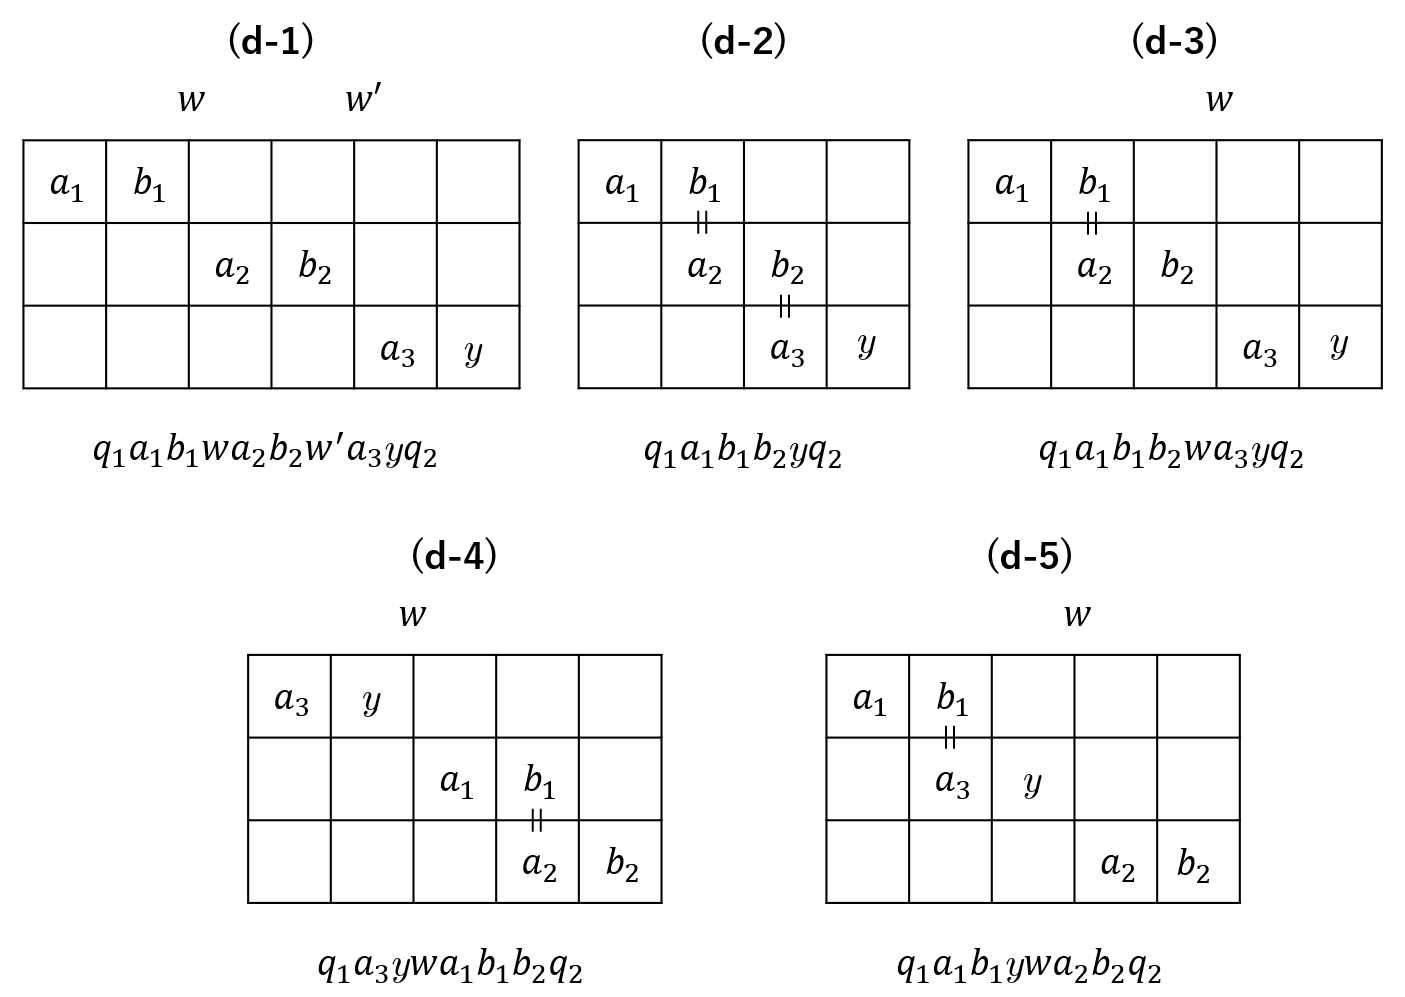
\includegraphics[width=\linewidth]{figs/Cases-d.png}
  \vspace{-1cm}
  \caption{(d)の場合分け}
  \label{d組み合わせ}
\end{figure}
    
Next, in the case of $C=a_{3}y$, we consider the following five cases (II-1)--(II-5):

\begin{tabular}{l}
(II-1) $q=q_{1}a_{1}b_{1}wa_{2}b_{2}w^{\prime}a_{3}yq_{2}$,\\
(II-2) $q=q_{1}a_{1}b_{1}b_{2}yq_{2}$ ($a_{2}=b_{1}$ and $a_{3}=b_{2}$),\\
(II-3) $q=q_{1}a_{1}b_{1}b_{2}wa_{3}yq_{2}$ ($b_{1}=a_{2}$),\\
(II-4) $q=q_{1}a_{3}ywa_{1}b_{1}b_{2}q_{2}$ ($b_{1}=a_{2}$),\\
(II-5) $q=q_{1}a_{1}b_{1}ywa_{2}b_{2}q_{2}$ ($b_{1}=a_{3}$).
\end{tabular}

\noindent
(II-1) Case of $q=q_{1}a_{1}b_{1}wa_{2}b_{2}w^{\prime}a_{3}yq_{2}$:
Assume that the following six equations (1),(2),(3),(1'),(2'),(3') are hold.
\begin{align*}
\textrm{(1)}~& p_{1} \preceq q_{1} & \textrm{(1')}~& p_{2} \preceq wa_{2}b_{2}w^{\prime}a_{3}yq_{2} \\
\textrm{(2)}~& p_{1} \preceq q_{1}a_{1}b_{1}w & \textrm{(2')}~& p_{2} \preceq w^{\prime}a_{3}yq_{2} \\
\textrm{(3)}~& p_{1} \preceq q_{1}a_{1}b_{1}wa_{2}b_{2}w^{\prime} & \textrm{(3')}~& p_{2} \preceq q_{2}
\end{align*}

%\noindent
If $|w|+1=|w^{\prime}|$, then $a_{1}b_{1}wa_{2}b_{2}w^{\prime}$ and $a_{1}b_{1}w$ are the suffix of $p_{1}$ from the above equations (2) and (3).
Since there exists a constant symbol $w_{1}$ such that $w^{\prime}=w_{1}w$ and $b_{2}w_{1}w=a_{1}b_{1}w$ hold,
then $b_{2}=a_{1}$.
Moreover, $wa_{2}b_{2}w^{\prime}a_{3}$ and $w^{\prime}a_{3}$ are the prefix of $p_{2}$ from the above equations (1') and (2').
Since there exists a constant symbol $w_{2}$ such that $w^{\prime}=ww_{2}$ and $wa_{2}b_{2}=ww_{2}a_{3}$ hold,
then $b_{2}=a_{3}$.
Thus, $a_{1} = a_{3}$ holds.
This contradicts the assumption of $a_{1} \ne a_{3}$.

%\noindent
If $|w|+1 < |w^{\prime}|$, then $a_{1}b_{1}wa_{2}b_{2}w^{\prime}$ and $a_{1}b_{1}w$ are the suffix of $p_{1}$ from the above equations (2) and (3).
Hence, $a_{1}b_{1}$ is the suffix of $w_{\prime}$.
Moreover, $wa_{2}b_{2}w^{\prime}a_{3}$ and $w^{\prime}a_{3}$ are the prefix of $p_{2}$ from the above equations (1') and (2').
Hence, there exist constant symbols $w_{1}$ and $w_{2}$ such that $w^{\prime}=w_{1}w$, $w^{\prime}=ww_{2}$ and $|a_{2}b_{2}w_{1}|=|w_{2}a_{3}|+1$ hold.
Thus, since the second-to-last symbol of $w_{1}$ is $a_{3}$, $a_{1}=a_{3}$ holds.
This contradicts the assumption of $a_{1} \ne a_{3}$.

%\noindent
If $|w^{\prime}|+1=|w|$, then $wa_{2}b_{2}w^{\prime}a_{3}$ and $w^{\prime}a_{3}$ are the prefix of $p_{2}$ from the above equations (1') and (2').
Since there exists a constant symbol $w_{1}$ such that $w=w^{\prime}w_{1}$ and $w^{\prime}w_{1}=w^{\prime}a_{3}$ hold, then $w_{1}=a_{3}$ holds.
Moreover, since $a_{1}b_{1}wa_{2}b_{2}w^{\prime}$ and $a_{1}b_{1}w$ are the suffix of $p_{1}$ from the above equations (2) and (3), 
there exists a constant symbol $w_{2}$ such that $w=w_{2}w^{\prime}$ and $|w_{1}a_{2}b_{2}w^{\prime}|=|a_{1}b_{1}w_{2}w^{\prime}|$ hold.
Hence, $w_{1}=a_{1}$ holds.
Thus, $a_{1}=a_{3}$ holds.
This contradicts the assumption of $a_{1}\ne a_{3}$.

%\noindent
If $|w| > |w^{\prime}|+1$, since $wa_{2}b_{2}w^{\prime}a_{3}$ and $w^{\prime}a_{3}$ are the prefix of $p_{2}$ from the above equations (1') and (2'),
there exists a constant string $w_{1}$ such that $w=w^{\prime}w_{1}$ and the first symbol of $w_{1}$ is $a_{3}$.
Moreover, since there exists a constant string $w_{2}$ such that $w=w_{2}w^{\prime}$ and $|w_{1}a_{2}b_{2}|=|a_{1}b_{1}w_{2}|$ hold,
$a_{1}b_{1}$ is the prefix of $w_{1}$.
Thus, $a_{3}=a_{1}$ holds.
This contradicts the assumption of $a_{1} \ne a_{3}$.
\smallskip

\noindent
(II-2) Case of $q=q_{1}a_{1}b_{1}b_{2}yq_{2}$ ($a_{2}=b_{1}$ and $a_{3}=b_{2}$):
Assume that the following six equations (1),(2),(3),(1'),(2'),(3') are hold.
\begin{align*}
\textrm{(1)}~& p_{1} \preceq q_{1} & \textrm{(1')}~& p_{2} \preceq b_{2}yq_{2} \\
\textrm{(2)}~& p_{1} \preceq q_{1}a_{1} & \textrm{(2')}~& p_{2} \preceq yq_{2} \\
\textrm{(3)}~& p_{1} \preceq q_{1}a_{1}b_{1} & \textrm{(3')}~& p_{2} \preceq q_{2}
\end{align*}

\noindent
From the above equations (2) and (3), $a_{1}b_{1}$ and $a_{1}$ are the suffix of $p_{1}$.
Hence, $b_{1}=a_{1}$ holds.
Thus, from the assumption of $b_{1}=a_{2}$, $a_{1}=a_{2}$ holds.
This contradicts the assumption of $a_{1} \ne a_{2}$.
\smallskip

\noindent
(II-3) Case of $q=q_{1}a_{1}b_{1}b_{2}wa_{3}yq_{2}$ ($b_{1}=a_{2}$):
Assume that the following six equations (1),(2),(3),(1'),(2'),(3') are hold.
\begin{align*}
\textrm{(1)}~& p_{1} \preceq q_{1} & \textrm{(1')}~& p_{2} \preceq b_{2}wa_{3}yq_{2} \\
\textrm{(2)}~& p_{1} \preceq q_{1}a_{1} & \textrm{(2')}~& p_{2} \preceq wa_{3}yq_{2} \\
\textrm{(3)}~& p_{1} \preceq q_{1}a_{1}b_{1}b_{2}w & \textrm{(3')}~& p_{2} \preceq q_{2}
\end{align*}

%\noindent
If $|w|=0$, that is $w$ is the empty string, then $a_{1}$ and $a_{1}b_{1}b_{2}$ are the suffix of $p_{1}$ from the above equations (2) and (3).
Hence, $a_{1}=b_{2}$ holds.
Moreover, since $b_{2}a_{3}$ and $a_{3}$ is the prefix of $p_{2}$, $b_{2}=a_{3}$ holds.
Thus, $a_{1}=a_{3}$ holds.
This contradicts the assumption of $a_{1} \ne a_{3}$.

%\noindent
If $|w| \ge 1$, since $a_{1}$ and $a_{1}b_{1}b_{2}w$ are the suffix of $p_{1}$ from the above equations (2) and (3),
the last symbol of $w$ is $a_{1}$.
Moreover, since $b_{2}wa_{3}$ and $wa_{3}$ are the prefix of $p_{2}$ from the above equations (1') and (2'),
the last symbol of $w$ is $a_{3}$.
Thus, $a_{1}=a_{3}$ holds.
This contradicts the assumption of $a_{1} \ne a_{3}$.
\smallskip

\noindent
(II-4) Case of $q=q_{1}a_{3}ywa_{1}b_{1}b_{2}q_{2}$ ($b_{1}=a_{2}$):
Assume that the following six equations (1),(2),(3),(1'),(2'),(3') are hold.
\begin{align*}
\textrm{(1)}~& p_{1} \preceq q_{1} & \textrm{(1')}~& p_{2} \preceq wa_{1}b_{1}b_{2}q_{2} \\
\textrm{(2)}~& p_{1} \preceq q_{1}a_{3}yw & \textrm{(2')}~& p_{2} \preceq b_{2}q_{2} \\
\textrm{(3)}~& p_{1} \preceq q_{1}a_{3}ywa_{1} & \textrm{(3')}~& p_{2} \preceq q_{2}
\end{align*}

\noindent
From the above equation (3), there exist regular patterns $p_{1}^{\prime}$と$p_{1}^{\prime\prime}$ such that $p_{1}=p_{1}^{\prime}p_{1}^{\prime\prime}$,$p_{1}^{\prime} \preceq q_{1}a_{3}$ and $p_{1}^{\prime\prime} \preceq ywa_{1}$ hold.
Hence, since $p=p_{1}xp_{2}=p_{1}^{\prime}p_{1}^{\prime\prime}xp_{2}\preceq q_{1}a_{3}p_{1}^{\prime\prime}xwa_{1}b_{1}b_{2}q_{2}=q_{1}a_{3}yxwa_{1}b_{1}b_{2}q_{2}\{ y := p_{1}^{\prime\prime}x \}=q \{ y := p_{1}^{\prime\prime}x \}$, then $p \preceq q$ holds.
Thus, this contradicts the assumption.
\smallskip

\noindent
(II-5) Case of $q=q_{1}a_{1}b_{1}ywa_{2}b_{2}q_{2}$ ($b_{1}=a_{3}$):
Assume that the following six equations (1),(2),(3),(1'),(2'),(3') are hold.
\begin{align*}
\textrm{(1)}~& p_{1} \preceq q_{1} & \textrm{(1')}~& p_{2} \preceq ywa_{2}b_{2}q_{2} \\
\textrm{(2)}~& p_{1} \preceq q_{1}a_{1} & \textrm{(2')}~& p_{2} \preceq wa_{2}b_{2}q_{2} \\
\textrm{(3)}~& p_{1} \preceq q_{1}a_{1}b_{1}yw & \textrm{(3')}~& p_{2} \preceq q_{2}
\end{align*}
\noindent
There exist regular patterns $q_{1}^{\prime}, q_{2}^{\prime}, q_{3}^{\prime}$ such that $q_{1}^{\prime}=q_{1}a_{1}b_{1}$, $q_{2}^{\prime}=yw$, $q_{3}^{\prime}=a_{2}b_{2}q_{2}$, from the above equation (3) $p_{1} \preceq q_{1}^{\prime}q_{2}^{\prime}$ and from the above equation (1') $p_{2} \preceq q_{2}^{\prime}q_{3}^{\prime}$ hold.
Moreover, since $q_{2}^{\prime}$ contains the variable symbol $y$, $p\preceq q$ holds from Theorem \ref{Sato1:Lemma9}.
This contradicts the assumption.
\end{proof}

